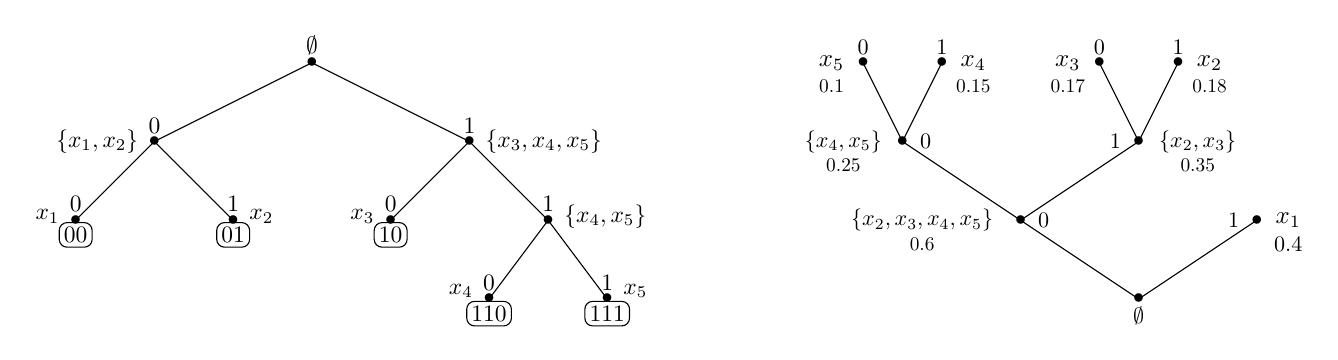
\begin{tikzpicture}%[xscale=3.5,yscale=3]
\shorthandoff{>}
%
% Codigo de Fano
\begin{scope}
\draw(0,0) node[scale=.8]{$\bullet$} node[above,scale=.85]{$\emptyset$};
%
% -----
%
\draw (0,0) -- (-2,-1) node[scale=.8]{$\bullet$} node[above,scale=.85]{$0$};
\draw (-2.1,-1) node[left,scale=.85]{$\{ x_1,x_2\}$};
%
\draw (0,0) -- (2,-1) node[scale=.8]{$\bullet$} node[above,scale=.85]{$1$};
\draw(2.1,-1) node[right,scale=.85]{$\{ x_3,x_4,x_5\}$};
%
% -----
%
\draw (-2,-1) -- (-3,-2) node[scale=.8]{$\bullet$} node[above,scale=.85]{$0$}
node[inner sep=2pt,outer sep=1pt,draw=black,below,scale=.85,rounded corners=1mm]{$00$};
\draw (-3.1,-1.95) node[left,scale=.85]{$\boldsymbol{x_1}$};
%
\draw (-2,-1) -- (-1,-2) node[scale=.8]{$\bullet$} node[above,scale=.85]{$1$}
node[inner sep=2pt,outer sep=1pt,draw=black,below,scale=.85,rounded corners=1mm]{$01$};
\draw (-.9,-1.95) node[right,scale=.85]{$\boldsymbol{x_2}$};
%
\draw (2,-1)-- (1,-2) node[scale=.8]{$\bullet$} node[above,scale=.85]{$0$}
node[inner sep=2pt,outer sep=1pt,draw=black,below,scale=.85,rounded corners=1mm]{$10$};
\draw (.9,-1.95) node[left,scale=.85]{$\boldsymbol{x_3}$};
%
\draw (2,-1)-- (3,-2) node[scale=.8]{$\bullet$} node[above,scale=.85]{$1$};
\draw (3.1,-1.95) node[right,scale=.85]{$\{ x_4 , x_5 \}$};
%
% -----
%
\draw (3,-2)-- (2.25,-3) node[scale=.8]{$\bullet$} node[above,scale=.85]{$0$}
node[inner sep=2pt,outer sep=1pt,draw=black,below,scale=.85,rounded corners=1mm]{$110$};
\draw (2.15,-2.9) node[left,scale=.85]{$\boldsymbol{x_4}$};
%
\draw (3,-2)-- (3.75,-3) node[scale=.8]{$\bullet$} node[above,scale=.85]{$1$}
node[inner sep=2pt,outer sep=1pt,draw=black,below,scale=.85,rounded corners=1mm]{$111$};
\draw (3.85,-2.9) node[right,scale=.85]{$\boldsymbol{x_5}$};
\end{scope}
%
%
% Codigo de Huffman
\begin{scope}[xshift=12cm]
\draw (-5,0) node[scale=.8]{$\bullet$} node[above,scale=.8]{$0$}
-- (-4.5,-1) node[scale=.8]{$\bullet$} node[right,scale=.8]{$\:\: 0$}
-- (-4,0) node[scale=.8]{$\bullet$} node[above,scale=.8]{$1$};
\draw(-5.4,0) node[scale=.9]{$\boldsymbol{x_5}$};
\draw(-5.4,-.3) node[scale=.7]{$0.1$};
\draw(-3.6,0) node[scale=.9]{$\boldsymbol{x_4}$};
\draw(-3.6,-.3) node[scale=.7]{$0.15$};
\draw(-5.25,-1) node[scale=.8]{$\{x_4,x_5\}$};
\draw(-5.25,-1.3) node[scale=.7]{$0.25$};
%
% -----
%
\draw (-2,0) node[scale=.8]{$\bullet$} node[above,scale=.8]{$0$}
-- (-1.5,-1) node[scale=.8]{$\bullet$} node[left,scale=.8]{$1\:\: $}
-- (-1,0) node[scale=.8]{$\bullet$} node[above,scale=.8]{$1$};
\draw(-2.4,0) node[scale=.9]{$\boldsymbol{x_3}$};
\draw(-2.4,-.3) node[scale=.7]{$0.17$};
\draw(-.6,0) node[scale=.9]{$\boldsymbol{x_2}$};
\draw(-.6,-.3) node[scale=.7]{$0.18$};
\draw(-.75,-1) node[scale=.8]{$\{x_2,x_3\}$};
\draw(-.75,-1.3) node[scale=.7]{$0.35$};
%
% -----
%
\draw (-4.5,-1) -- (-3,-2) node[scale=.8]{$\bullet$} node[right,scale=.8]{$\:\: 0$} -- (-1.5,-1);
\draw(-4.25,-2) node[scale=.8]{$\{x_2,x_3,x_4,x_5\}$};
\draw(-4.25,-2.3) node[scale=.7]{$0.6$};
%
% -----
%
\draw (-3,-2) -- (-1.5,-3) node[scale=.8]{$\bullet$} node[below,scale=.8]{$\emptyset$}
-- (0,-2) node[scale=.8]{$\bullet$} node[left,scale=.8]{$1\:\:$};
\draw(.4,-2) node[scale=.9]{$\boldsymbol{x_1}$};
\draw(.4,-2.3) node[scale=.8]{$0.4$};
\end{scope}
\end{tikzpicture}